Cryogenic temperatures for the setup are realized using a circulating helium system by Oxford Instruments\footnote{Oxford Instruments Microstat HiRes2}. The schematic overview is shown in figure \ref{fig:cryo_setup}.

\begin{figure}[H]
\centering
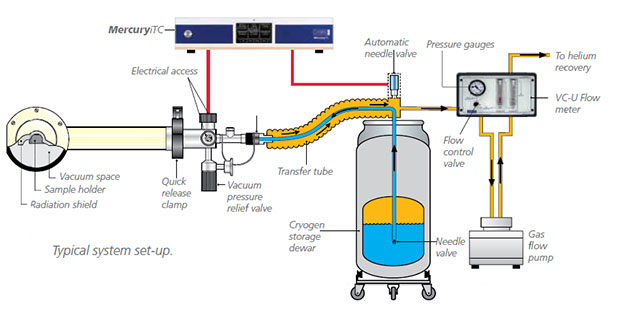
\includegraphics[scale=0.7]{cryostat.jpg}
\caption{An overview of the cryogenic setup. Picture taken from Oxford Intruments product webpage.}
\label{fig:cryo_setup}
\end{figure}

The cryostat is connected to a vacuum pump, such that a vacuum inside the cryostat can be achieved. We normally reach a vacuum of \SI{1e-6}{\milli\bar}, which is acceptable taking our cleaning and assemble procedure into account. Between the vacuum pump an the cryostat we have connected an extra tube enclosed in a heavy concrete block placed on vibration damping foam blocks, to prevent vibrations from the pump the travel to the cryostat. Even though the concrete block sounds and is low tech, it is quite crucial to the setup. Inside the cryostat a cold finger, is where we attach the sample holder. The cold finger is connected to the liquid helium by a transfer tube which is inserted into the dewar and then the cryostat. The transfer tube has two channels of flow. The one (inner) from the dewar to cold finger and the other (outer) from the cold finger to an exhaust. A gas pump and a flow meter are responsible for the continuous flow through the cycle. The amount of helium flow can be regulated by a needle valve on the transfer tube and or by a control valve connected to pressure gauge on the flow meter.

To measure the temperature inside the cryostat a temperature sensor is included in the cold finger. More temperature sensors could be added, for example in the sample holder close to the sample, but we ran out of sensors. The temperature can be stabilized by a heater. The cryostat's specified minimum temperature is around the temperature of liquid helium \SI{4.2}{\kelvin}.